% rubber: rules ./rules.ini
\documentclass[11pt]{article}
\usepackage{a4wide}
\usepackage{styles/sujet_iut}

\usepackage{multicol}
\usepackage{moreverb}
\usepackage{vmargin}
\usepackage{parskip}

\titreEpreuve{ASR2 Syst�me\\\vspace{0.2cm}
Contr�le continu}
\dateEpreuve{9 mai 2011}
\publicEpreuve{Semestre 2}

\setmarginsrb{2cm}{0.5cm}{3cm}{1cm}{0cm}{1cm}{0cm}{0cm}
\newcounter{cq}
\setcounter{cq}{1}

\begin{document}
\maketitle

\vspace{0.2cm}
Sans documents, 35 minutes, \textbf{marquez votre nom en haut de la feuille}. 

On consid�re les 6 processus suivants dans un syst�me non pr�emptif :

\begin{center}
\small
\begin{tabular}{c c c c}
  Processus  & Instant d'arriv�e & Dur�e & Priorit� \\
  \hline
  P1 & 0  & 3  & 1 \\
  P2 & 1  & 24 & 2 \\
  P3 & 1  & 8  & 3 \\
  P4 & 8  & 4  & 2 \\
  P5 & 10 & 2  & 5 \\
  P6 & 16 & 2  & 3 \\
\end{tabular}
\end{center}

%\newpage
Donnez l'ordre d'ex�cution des processus et calculez le temps de service moyen pour
les politiques d'ordonnancement suivantes~:
\boite{\thecq.\stepcounter{cq}  FIFO~:\\
\vspace{2.5cm}\\
\thecq.\stepcounter{cq} Plus Court Temps d'Ex�cution~: \\
\vspace{2.5cm}\\
\thecq.\stepcounter{cq} avec priorit�~:\\
}{2.5}

%% Idem pour la politique d'ordonnancement  
%% \boite{\thecq.\stepcounter{cq}}{2.5}

%% Idem une politique d'ordonnancement avec priorit�s.
%% \boite{\thecq.\stepcounter{cq}}{2.5}


Qu'est ce qu'un syst�me d'exploitation?
Que g�re t-il?
\boite{\thecq.\stepcounter{cq}}{2}
 
Qu'est ce qu'un processus?
\boite{\thecq.\stepcounter{cq}}{1.5}

Nommez et d�crivez les diff�rents �tats d'un processus.
\boite{\thecq.\stepcounter{cq}}{4}

Un syst�me multi-t�che peut �tre pr�emptif ou non pr�emptif.\\
Expliquez le mode de fonctionnement de ces deux types de syst�mes. 
\boite{\thecq.\stepcounter{cq}}{4}

%% D�finissez en quelques mots ce qu'est l'ordonnancement. %
% \boite{\thecq.\stepcounter{cq}}{3}




On consid�re 3 processus de comportements r�p�titifs suivants~:
\begin{itemize}
\item P1 calcule 10ms puis effectue une op�ration d'entr�e-sortie (E/S) pendant 10ms.  
\item P2 effectue 5ms de calcul, une E/S de 10ms, 25ms de calcul, une E/S de 10ms 
\item P3 calcule 30ms puis une E/S de 20ms. 
\end{itemize}
Les op�rations d'E/S sont effectu�es de fa�on s�quentielle.
Le sch�ma suivant repr�sente le d�but de l'ordonnancement des processus P1, P2,
P3.  
\begin{figure}[h!]
  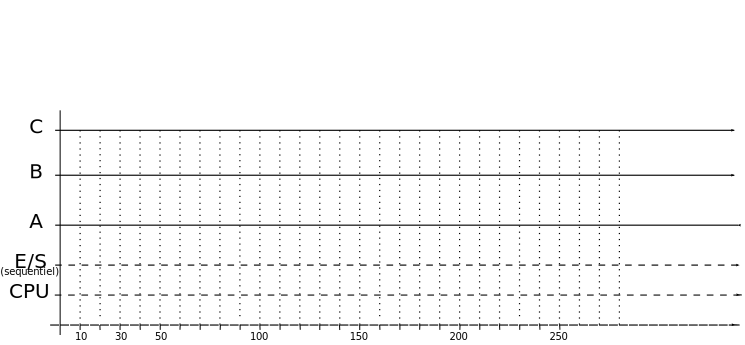
\includegraphics[width=\linewidth]{fig/ordo}
\end{figure}

Que pouvez vous dire du syst�me et de la politique d'ordonnancement employ�e.\\
Justifiez vos r�ponses
\boite{\thecq.\stepcounter{cq}}{5}

\end{document}


% LocalWords:  rubber rules t-il cq multi-t�che d'Ex�cution d'entr�e-sortie d'E
% LocalWords:  width
